\begin{center}
  \scalebox{1.0}{
    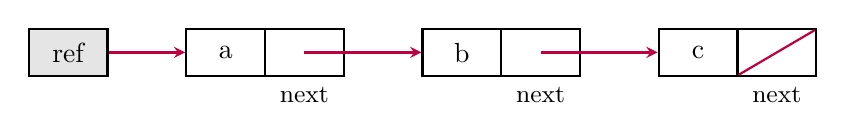
\begin{tikzpicture}[]
      \coordinate (origo) at (0mm,-6cm);
      
      \tikzstyle{cell} = [
        rectangle,
        draw=black,
        thick,
        anchor=west,
        minimum width=10mm,
        minimum height=6mm,
      ]
      \tikzstyle{celllabel} = [
        draw=none,
        anchor=north,
        align=center
      ]
      
      \tikzstyle{arrow} = [thick,->,>=stealth, draw=purple]
      
      % object
      \node[cell,fill=black!10] (cellFirst) at ([xshift=0mm] origo) {ref};
      
      % link 1
      \node[cell] (cell1data) at ([xshift=20mm] origo) {a};
      \node[cell] (cell1next) at ([xshift=30mm] origo) {};
      \node[celllabel] (cell1nextLabel) at ([xshift=0mm] cell1next.south) {\small next};
      
      % link 2
      \node[cell] (cell2data) at ([xshift=50mm] origo) {b};
      \node[cell] (cell2next) at ([xshift=60mm] origo) {};
      \node[celllabel] (cell2nextLabel) at ([xshift=0mm] cell2next.south) {\small next};
      
      % link 1
      \node[cell] (cell3data) at ([xshift=80mm] origo) {c};
      \node[cell] (cell3next) at ([xshift=90mm] origo) {};
      \node[celllabel] (cell3nextLabel) at ([xshift=0mm] cell3next.south) {\small next};
      
      % forward
      \draw[arrow] (cellFirst.east) -- (cell1data.west);
      \draw[arrow] (cell1next.center) -- (cell2data.west);
      \draw[arrow] (cell2next.center) -- (cell3data.west);
      
      % null
      \draw[overlay,thick,draw=purple] ([xshift=-0.3mm,yshift=-0.3mm] cell3next.north east) -- ([xshift=0.3mm,yshift=0.3mm] cell3next.south west);
    \end{tikzpicture}
  }
\end{center}
